\documentclass[12pt]{article}
\usepackage[a4paper, margin=0.75in]{geometry}
\usepackage[document]{ragged2e}
\usepackage{graphicx}
\usepackage{subcaption}
\usepackage{placeins}
\graphicspath{ {./images/} }
\usepackage{enumerate}
\usepackage{framed}
\usepackage{amsmath,amsfonts,amsthm,thmtools,amssymb,mathtools,commath}
\usepackage{physics}
\usepackage{tikz}
\usetikzlibrary{mindmap}
\usepackage{caption}
\usepackage{xcolor}
\usepackage[most]{tcolorbox}
\usepackage{cleveref}


%%%%%%%%%%%%%%%%
%  Definition  %
%%%%%%%%%%%%%%%%
\tcbuselibrary{theorems,skins,hooks}
\newtcbtheorem[number within=subsection]{definition}{Definition}%
{
    % theorem style=definition,
    enhanced,
	before skip=2mm,after skip=2mm, colback=cyan!5,colframe=cyan!80!black,boxrule=0.5mm,
	attach boxed title to top left={xshift=1cm,yshift*=1mm-\tcboxedtitleheight},
	boxed title style={frame code={
					\path[fill=cyan]
					([yshift=-1mm,xshift=-1mm]frame.north west)
					arc[start angle=0,end angle=180,radius=1mm]
					([yshift=-1mm,xshift=1mm]frame.north east)
					arc[start angle=180,end angle=0,radius=1mm];
					\path[left color=cyan!30!black,right color=cyan!30!black,
						middle color=cyan!50!black]
					([xshift=-2mm]frame.north west) -- ([xshift=2mm]frame.north east)
					[rounded corners=1mm]-- ([xshift=1mm,yshift=-1mm]frame.north east)
					-- (frame.south east) -- (frame.south west)
					-- ([xshift=-1mm,yshift=-1mm]frame.north west)
					[sharp corners]-- cycle;
				},interior engine=empty,
		},
	fonttitle=\bfseries,
	title={#2},#1
}{def}


%%%%%%%%%%%%%
%  Theorem  %
%%%%%%%%%%%%%
\tcbuselibrary{theorems,skins,hooks}
\newtcbtheorem[use counter from=definition]{theorem}{Theorem}%
{
    theorem style=plain,
    enhanced,
    colframe=green,
    boxrule=1pt,
    titlerule=0mm,
    toptitle=1mm,
    bottomtitle=1mm,
    fonttitle=\bfseries,
    fontupper=\mdseries\itshape,
    coltitle=green!30!black,
    colbacktitle=cyan!15!white,
    colback=green!10,
    description font=\bfseries\sffamily
}{thrm}


%%%%%%%%%%%%%%
% Corollary  %
%%%%%%%%%%%%%%
 \tcbuselibrary{theorems,skins}
 \newtcbtheorem[use counter from=theorem]{corollary}{Corollary}%
 {
    theorem style=plain,
    enhanced,
    colframe=green,
    frame hidden,
    titlerule=0mm,
    toptitle=1mm,
    bottomtitle=1mm,
    fonttitle=\bfseries,
    fontupper=\mdseries\itshape,
    coltitle=green!30!black,
    colbacktitle=cyan!15!white,
    colback=green!10,
    description font=\bfseries\sffamily
 }{corl}


%%%%%%%%%%%%%
%  Example  %
%%%%%%%%%%%%%
\tcbuselibrary{theorems,skins,hooks}
\newtcbtheorem[number within=section]{example}{Example}%
{
	enhanced,
	breakable,
	colback = gray!5,
	frame hidden,
	boxrule = 0sp,
	borderline west = {2pt}{0pt}{gray},
	sharp corners,
	detach title,
	before upper = \tcbtitle\par\smallskip,
    coltitle=gray!70!black,
	fonttitle = \bfseries\sffamily,
	description font = \mdseries\bfseries
}
{xmp}


%%%%%%%%%%%%%%
%  Exercise  %
%%%%%%%%%%%%%%
\tcbuselibrary{theorems,skins,hooks}
\newtcbtheorem[number within=section]{exercise}{Exercise}%
{
    enhanced,
    breakable,
    colback=black!5,
    colframe=black!30,
    left=0.5em,
    before skip=10pt,
    after skip=10pt,
    boxrule=0pt,
    boxsep=0pt,
    arc=0pt,
    outer arc=0pt,
    borderline west={3pt}{0pt}{black!30},
}{exc}

%%%%%%%%%%
%  Note  %
%%%%%%%%%%
\usetikzlibrary{arrows,calc,shadows.blur}
\tcbuselibrary{skins}
\newtcolorbox{note}[1][]{%
	enhanced jigsaw,
	colback=gray!20!white,%
	colframe=gray!80!black,
	size=small,
	boxrule=1pt,
	title=\textbf{Note:-},
	halign title=flush center,
	coltitle=black,
	breakable,
	drop shadow=black!50!white,
	attach boxed title to top left={xshift=1cm,yshift=-\tcboxedtitleheight/2,yshifttext=-\tcboxedtitleheight/2},
	minipage boxed title=1.5cm,
	boxed title style={%
			colback=white,
			size=fbox,
			boxrule=1pt,
			boxsep=2pt,
			underlay={%
					\coordinate (dotA) at ($(interior.west) + (-0.5pt,0)$);
					\coordinate (dotB) at ($(interior.east) + (0.5pt,0)$);
					\begin{scope}
						\clip (interior.north west) rectangle ([xshift=3ex]interior.east);
						\filldraw [white, blur shadow={shadow opacity=60, shadow yshift=-.75ex}, rounded corners=2pt] (interior.north west) rectangle (interior.south east);
					\end{scope}
					\begin{scope}[gray!80!black]
						\fill (dotA) circle (2pt);
						\fill (dotB) circle (2pt);
					\end{scope}
				},
		},
	#1,
}


\title{
    \textbf{Experiment 5}\\
    \textbf{\large Experiments on Class B, Class B push-pull, Class AB, and Class C Multistage Amplifier}
}

\author{
    Turja Roy\\
    2108052
}
\date{February 20, 2024}

\begin{document}
\maketitle

\section{Objective}
\begin{enumerate}
    \item To study the working principle of a Class B Multistage Amplifier.
    \item To study the working principle of a Class AB Multistage Amplifier.
    \item To study the working principle of a Class B push-pull Multistage Amplifier.
    \item To study the working principle of a Class C Multistage Amplifier.
    \item To measure the voltage gain of the amplifiers.
    \item To measure the current gain of the amplifiers.
    \item To measure the power gain of the amplifiers.
\end{enumerate}

\section{Apparatus}
\begin{enumerate}
    \item Transistors (2N3904 npn) - 2
    \item Resistors (220 $\Omega$, 1.2 k$\Omega$, 3.6 k$\Omega$, 20 k$\Omega$, 10 k$\Omega$)
    \item Capacitors (10 $\mu$F) - 3
    \item DC Power Supply (0-30V)
    \item Function Generator
    \item Oscilloscope
    \item Multimeter
    \item Breadboard, Connecting wires, etc.
\end{enumerate}

\section{Circuit Diagram}
In the following page is given the circuit diagram for the Class A Amplifier. The multistage amplifier was built by connecting two amplifier circuits through the capacitor $C_5$. The output of the first amplifier ($Q_1$) acts as the input of the second amplifier ($Q_3$). The 10k $\Omega$ is the load resistor in the circuit. Oscilloscope has been connected in the shown way to get the input and output curves.

\begin{figure}[!htpb]
    \centering
    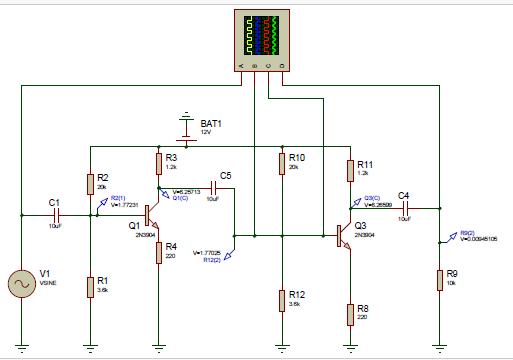
\includegraphics[width=0.7\textwidth]{Circuit Diagram.png}
    \caption{Class A Amplifier Circuit Diagram}
\end{figure}

\FloatBarrier
\section{Result Analysis}
A multi stage amplifier amplifies a signal in multiple stages. The input of the first stage is amplified and collected at at the output terminal and that output becomes the input for the second stage. This is how a signal gets amplified in multiple stages. The overall voltage gain of the signal is going to be the multiplication of the voltage gain of each of these circuits.

\subsection{Data Table for Class A Multistage Amplifier}
\bgroup
\def\arraystretch{1.5}
\begin{table}[h!]
    \centering
    \caption{Data table for Class A multistage amplifier}
    \begin{tabular}{|c|c|c|c|c|c|c|}
        \hline
        \multicolumn{7}{|c|}{\textbf{Theoretical Data}} \\
        \hline
        $V_{in}$ (mV) & $V_{out}$ (mV) & $I_{in}$ ($\mu$A) & $I_{out}$ ($\mu$A) & $A_V$ & $A_I$ & $A_P$ \\ \hline
        50 & 620 & 19.2 & 61.81 & 12.4 & 3.22 & 39.93 \\ \hline\hline
        \multicolumn{7}{|c|}{\textbf{Simulation Data}} \\
        \hline
        $V_{in}$ (mV) & $V_{out}$ (mV) & $I_{in}$ ($\mu$A) & $I_{out}$ ($\mu$A) & $A_V$ & $A_I$ & $A_P$ \\ \hline
        50 & 617 & 19.2 & 61.7 & 12.34 & 3.21 & 39.61 \\ \hline\hline
        \multicolumn{7}{|c|}{\textbf{Practical Data}} \\
        \hline
        $V_{in}$ (mV) & $V_{out}$ (mV) & $I_{in}$ ($\mu$A) & $I_{out}$ ($\mu$A) & $A_V$ & $A_I$ & $A_P$ \\ \hline
        50 & 572 & 15.2 & 65.7 & 11.44 & 4.32 & 49.42 \\ \hline\hline
        \multicolumn{7}{|c|}{\textbf{Error Analysis (Simulation vs Practical Data)}} \\
        \hline
        $V_{in}$ \% & $V_{out}$ \% & $I_{in}$ \% & $I_{out}$ \% & $A_V$ \% & $A_I$ \% & $A_P$ \% \\ \hline
        0 & 10.86 & 20.83 & 6.48 & 0.38 & 34.58 & 24.77 \\ \hline
    \end{tabular}
\end{table}
\egroup

\subsection{Class A Multistage Amplifier Input and Output Graphs}

\begin{figure}[h!]
    \centering
    \begin{subfigure}{0.45\textwidth}
        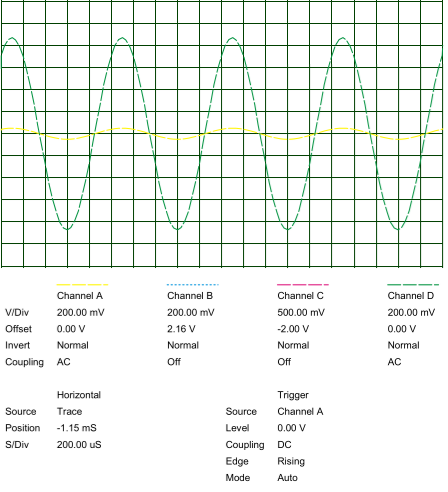
\includegraphics[width=\textwidth]{Simulated_graph.png}
        \caption{Simulated Graph}
    \end{subfigure}
    \begin{subfigure}{0.45\textwidth}
        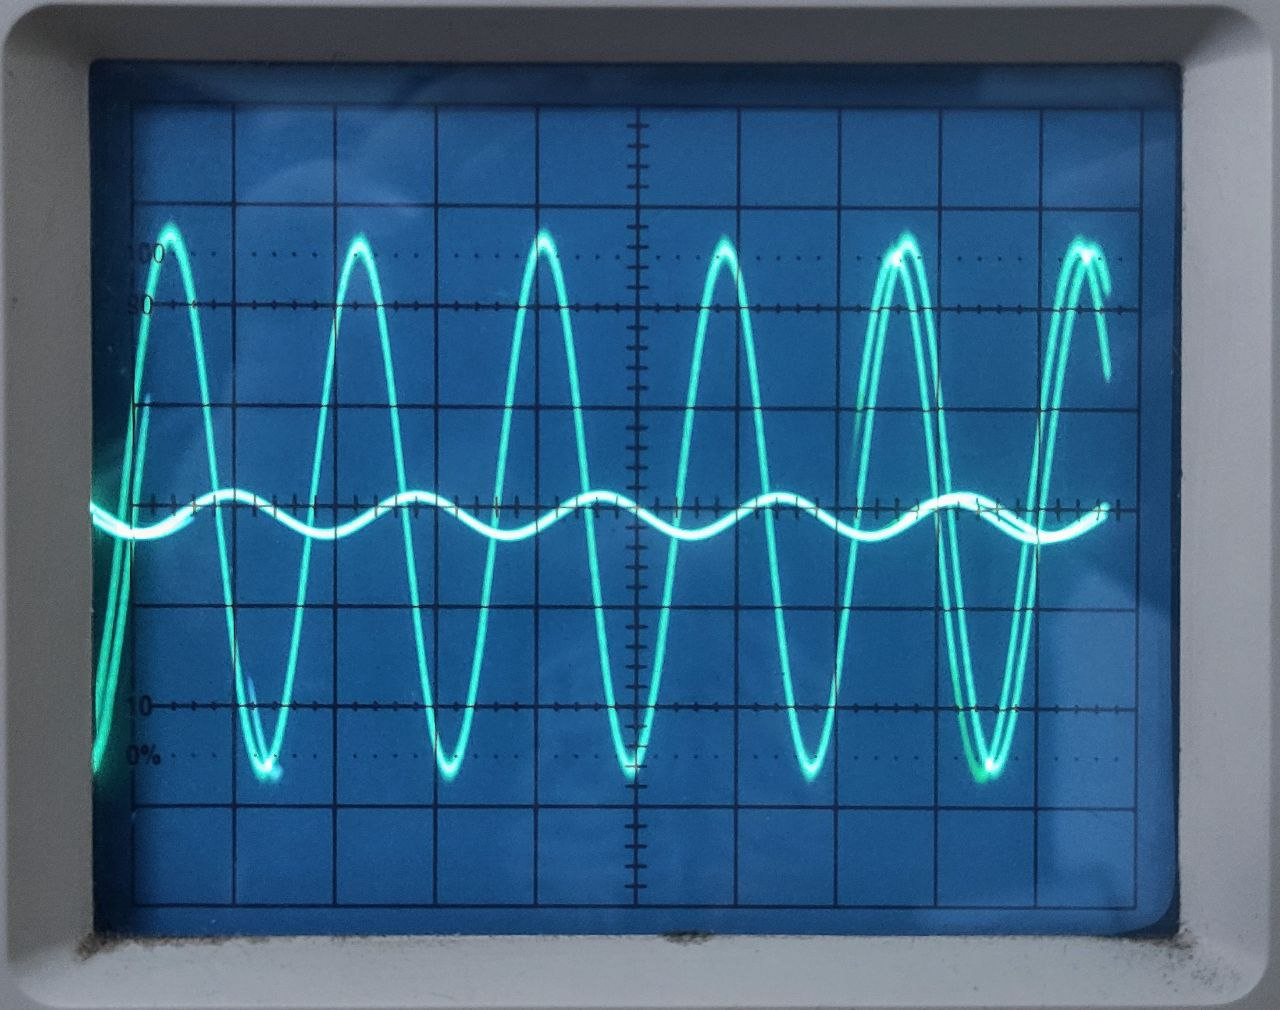
\includegraphics[width=\textwidth]{Practical_graph.jpg}
        \caption{Experimental Graph}
    \end{subfigure}
    \caption{Simulated and Practical Input and Output Graphs for Class A Multistage Amplifier}
\end{figure}

In the simulated graph (Figure 2-a), the yellow and the green dashed lines show the input and output curves respectively. In the practical graph (Figure 2-b), the shorter amplitide curve is input graph and the other one is output curve.


\section{Discussion}
The experiment was conducted to observe the amplification of a signal in multiple stages. Error had been measured between the simulated data and the practical data. The error analysis shows that the accuracy of the practical data is roughly within the range of 75\% to 90\%. The theoretical, simulation and practical data had some discripancies. One of the possible reason for this was that in the theoretical and simulated data, the internal resistance of wires and other equipments were considered negligible.

\end{document}
